\chapter{Contexte général du projet}
\label{chap:Contexte général du projet}



Ce chapitre situe mon projet de fin d’études dans son environnement organisationnel et contextuel. Il commence par une présentation de l’organisme d’accueil, SQLI Maroc. Ensuite, il détaille la problématique ayant conduit à la réalisation de ce projet ainsi que les objectifs visés. Enfin, la méthodologie adoptée pour mener à bien le projet est abordée.

\newpage


\section{Présentation de l’entreprise d’accueil SQLI}

Cette section initiale met en lumière le Groupe SQLI en mettant l’accent sur ses activités clés, son
chiffre d’affaires ainsi que ses clients. EEnsuite, l'accent sera mis sur SQLI Maroc, en mettant en avant ses valeurs fondamentales.

\subsection{Groupe SQLI}

\begin{figure}[h]
    \centering
    
\includegraphics[scale=0.7]{Logos/SQLI_LOGO.png} % Replace with the actual filename of the IBM logo image
    \caption{Logo de SQLI \cite{SQLI}}
    \label{fig:LogoSQLI}
\end{figure}

SQLI est une entreprise européenne de services numériques fondée en 1990 par Jean Rouveyrol et Alain Lefebvre. Elle se spécialise dans la conception, le développement et le déploiement de solutions digitales
visant à créer des expériences unifiées \cite{SQLI}. Avec un effectif de 2400 collaborateurs répartis dans 13 pays,
SQLI bénéficie d’une présence internationale solide.

Le succès de SQLI Digital Experience repose sur des valeurs fondamentales telles que la créativité, l'engagement et l'audace visionnaire. Ces valeurs imprègnent chaque aspect de l'entreprise, permettant de repousser les frontières de l'innovation et de concevoir des expériences digitales uniques et captivantes. \cite{valeurSQLI}

\subsubsection{Activités du groupe}

Le groupe SQLI propose une gamme étendue de services pour accompagner les entreprises dans leur transformation numérique. Il inclut l'e-commerce, créant et optimisant des plateformes de vente en ligne performantes. Il offre également des plateformes d'expérience, conçues pour offrir des interactions utilisateur exceptionnelles. En matière de technologie et de transformation, il aide les entreprises à moderniser leurs infrastructures et leurs processus. Ses services de data et insights permettent d'exploiter les données de manière stratégique, tandis que son expertise en marketing digital et design améliore la visibilité et l'attrait des marques. Enfin, son conseil digital guide les entreprises dans l'élaboration et la mise en œuvre de leur stratégie numérique globale, assurant ainsi une transformation digitale réussie. \cite{SQLI}

\subsubsection{Chiffres Clés du groupe}

Les chiffres clés suivants présentent la situation actuelle de SQLI :

\begin{itemize}
    \item[$\bullet$] Fort de 33 ans d’expérience et d’innovation, SQLI fonde son développement sur une expertise technologique de pointe et une politique de veille intensive.
    \item[$\bullet$] SQLI emploie plus de 2400 collaborateurs répartis dans 13 pays, notamment la France, l'Angleterre, la Suède, les Pays-Bas, l'Espagne, l'Allemagne, la Belgique, le Luxembourg, la Suisse et le Maroc.
    \item[$\bullet$] En 2022, le groupe SQLI a atteint un chiffre d’affaires de 251,2 millions de dollars. Ce succès est le résultat d'une offre bien alignée sur les attentes du marché et d'une reprise progressive de la demande de services informatiques.
    \vspace{0.5cm}
\end{itemize}

\begin{figure}[H]
    \centering
    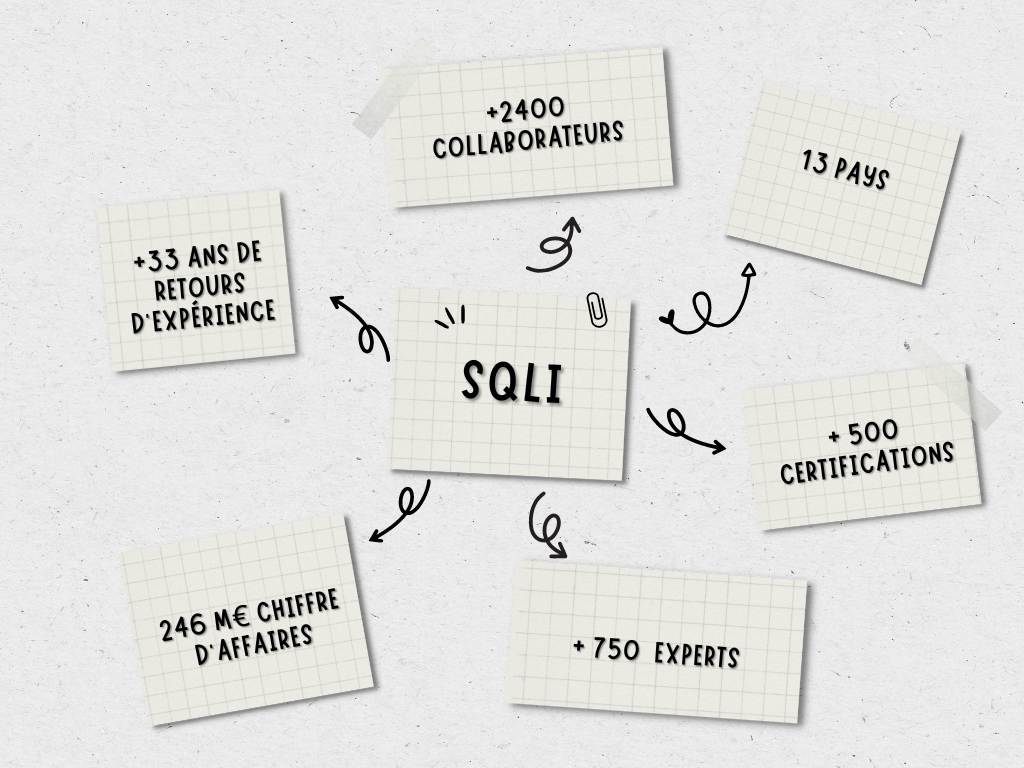
\includegraphics[width=10cm]{Figures/cle chiffre.png} % Replace with the actual filename of the IBM logo image
    \caption{Chiffre Clés de SQLI}
\end{figure}

\subsubsection{Clients du groupe}

SQLI collabore avec une vaste gamme de clients provenant de divers secteurs, y compris l'automobile, la distribution, la banque et l'assurance, le luxe et la mode, la santé, l'industrie et l'énergie, ainsi que les télécommunications. Les grandes entreprises internationales et les organisations locales font appel à SQLI pour ses solutions digitales innovantes, allant de l'optimisation des plateformes d'e-commerce à la transformation numérique des services financiers, en passant par la création d'expériences utilisateur uniques pour les marques de luxe et la digitalisation des processus industriels. Grâce à sa capacité à répondre aux besoins spécifiques de chaque secteur, SQLI bâtit des partenariats solides et durables avec ses clients (voir \textit{Figure~\ref{fig:client}})

\begin{figure}[H]
    \centering
    
\includegraphics[width=15cm]{Figures/sqli partenaire .png} % Replace with the actual filename of the IBM logo image
    \caption{Clients du SQLI \cite{SQLI}}
    \label{fig:client}
\end{figure}


\subsection{SQLI Maroc}

SQLI Maroc, créée en 2003 à Rabat par Eric Chanal, représente le centre de Delivery et d'Innovation du Groupe SQLI. Bénéficiant d'une solide expertise et d'une grande expérience, l'entreprise est présente sur trois sites stratégiques : Rabat, où j'ai eu l'opportunité d'effectuer notre stage PFE, Oujda et Casablanca. Le tableau suivant représente sa fiche technique:



% l'ajoute de titre de tableau avec space between titre de tab et le tab
% \captionsetup{type=table}

% \vspace{0.3cm}
% tab
\begin{center}
    \captionsetup{type=table}
    \label{tab:fiche}
    \vspace{0.3cm}
    \begin{tabularx}{17cm}{|X|X|}
      \hline
     \textbf{Dénomination sociale}  & \textbf{SQLI Digital Experience} \\
      \hline
     {Année de fondation} & 2003  \\
      \hline
      {Fondateur} & Eric Chanal  \\
      \hline
     {Siège social} & Rabat, Maroc\\
     \hline  
     {Activité} & Conseil en systèmes et logiciels informatiques.\\
      \hline  
     {Effectif des employés} & Plus de 900 collaborateurs.\\
      \hline
     {Sites d'implantation} & Rabat, Oujda et Casablanca.\\
      \hline
    \end{tabularx}
    \captionof{table}{Fiche technique de SQLI Maroc}
    \end{center}
    

  SQLI Maroc comprend principalement deux structures essentielles, présentées dans la \textit{Figure~\ref{fig:departement}}, à savoir :

\begin{enumerate}
    \item \textbf{SQLI WAX INTERRACTIVE} : accompagne les clients dans leur transition vers la digitalisation afin de renforcer leur positionnement sur le marché. Cette entité intervient principalement sur le plan stratégique en collaborant étroitement avec les clients.
     \item \textbf{SQLI ENTREPRISE} : Cette entité est chargée de la mise en œuvre des systèmes d'information pour les clients. Elle se compose de plusieurs Business Units spécialisées dans différents domaines :
\begin{itemize}

    \item \textbf{E-commerce/ JAVA EE} : Se focalise sur la création et la mise en place de sites de e-commerce ainsi que sur le développement d’applications utilisant la technologie Java EE.
    \item \textbf{Mobile/Front} : Se spécialise dans le développement d’applications mobiles et l’interface utilisateur (front-end) pour les clients.
    \item \textbf{Microsoft} : S'occupe de la réalisation d’applications basées sur les technologies Microsoft.
    \item \textbf{Agency} : Joue un rôle transversal en assurant la conception de l’interface utilisateur (front-end) pour toutes les autres Business Units.
    \item \textbf{Delivery} : Se charge de la gestion des livraisons et des recettes auprès des clients.
\end{itemize}
\end{enumerate}
\vspace{0.5cm}
\begin{figure}[H]  
  \centering  
  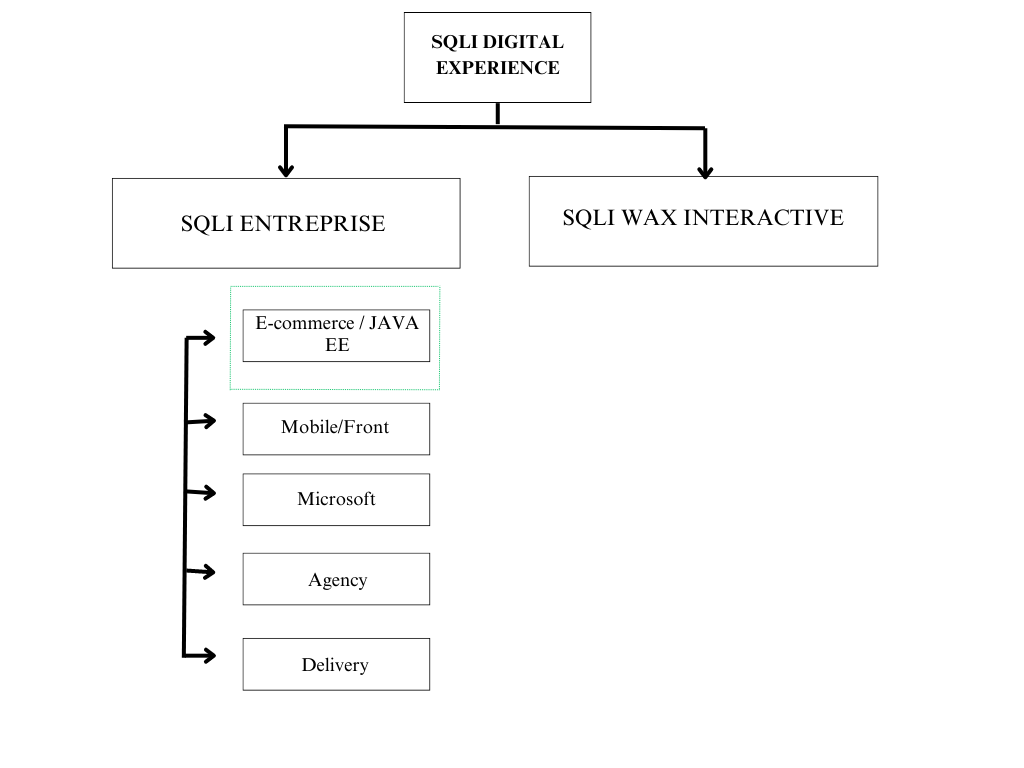
\includegraphics[width=14cm]{Figures/departement.png}
  \caption{Départements de SQLI}
  \label{fig:departement}
\end{figure}


Mon stage de fin d'études s'est déroulé dans le département Java JEE, qui regroupe plusieurs projets destinés à de grandes entreprises clientes.


\section{Présentation du projet}

\subsection{Cadre du projet et problématique}

Dans le cadre d'un projet e-commerce pour un client, l'objectif est d'améliorer et d'optimiser sa plateforme actuelle. Il est indispensable de mettre à jour régulièrement cette plateforme, qui joue un rôle crucial dans les activités commerciales en ligne du client, afin de maintenir sa compétitivité et de répondre aux exigences du marché.

Pour cette amélioration, le travail inclut la correction de divers bugs qui affectent la performance et la fiabilité du système. La résolution de ces bugs est cruciale pour garantir une expérience utilisateur fluide et sans interruptions.

En parallèle, l'intégration de nouvelles fonctionnalités est nécessaire pour enrichir l'offre de la plateforme. L'un des changements majeurs est l'intégration de la méthode de paiement Payconiq, destinée spécifiquement au marché belge. Différents défis se posent lors de cette intégration, tels que la compatibilité avec l'architecture existante, la gestion des dépendances et l'assurance que cette nouvelle fonctionnalité ne provoque pas de régressions ou de nouveaux bugs.

L'enjeu majeur consiste donc à corriger les bugs existants tout en intégrant Payconiq de manière efficace, en maintenant la stabilité et la performance globale de la plateforme.

 \subsection{Objectifs du projet}

 Dans le cadre de ce projet, je participerai activement aux diverses activités de l'équipe, contribuant à la fois au développement des fonctionnalités demandées par le client et à l'amélioration continue du système. Les objectifs spécifiques de mon intervention sont les suivants :

 \begin{itemize}
    \item[$\bullet$] \textbf{Intégrer un nouveau mode de paiement, Payconiq, pour le marché belge :} 
    
    Analyser et comprendre l'architecture existante pour intégrer Payconiq, tout en gérant les dépendances et en garantissant la compatibilité avec les autres modules de la plateforme, conformément aux spécificités techniques du marché belge. Cela inclut la configuration, le développement, et des tests rigoureux pour garantir une intégration fluide dans les différents flux de paiement existants.

    \item[$\bullet$] \textbf{Assurer les livraisons dans différents environnements (DEV, INTx, UAT, PRD) :} 
    
    Garantir le bon fonctionnement du code dans chacun de ces environnements, conformément aux exigences de stabilité et de performance. Cela comprend des tests approfondis pour s'assurer que les nouvelles fonctionnalités et intégrations sont stables et opérationnelles avant la mise en production.

    \item[$\bullet$] \textbf{Respecter les meilleures pratiques, les normes, et l'architecture du projet :} 
    
    Assurer la cohérence du code et la stabilité du projet en adhérant aux normes et pratiques de développement établies. Cela inclut le respect des principes d'architecture définis, l'application des bonnes pratiques de codage, et la proposition de solutions conformes aux standards en vigueur au sein de l'équipe.

    \item[$\bullet$] \textbf{Analyser et corriger les bugs détectés :}
    
    Assurer la maintenance corrective du système en identifiant, analysant, et résolvant les bugs remontés par les équipes ou découverts lors des tests, afin de minimiser leur impact sur le fonctionnement global de la plateforme.

\end{itemize}

 %%%%%%%%%%%%%%%%%%%% SECTION 4 %%%%%%%%%%%%%%%%%%%%%%%
\section{Conduite de projet}

\subsection{Présentation des Équipes du Projet}

Après ma période de formation, j’ai intégré une première équipe en tant que stagiaire backend. Cette équipe était responsable des aspects liés à la recherche, aux lunettes et à la mode pour le projet Chanel. À mon arrivée, l'équipe se concentrait sur le Plan 99.5, visant à analyser les bugs, nettoyer les logs, corriger les erreurs et refactoriser le code. La structure de cette équipe est illustrée dans la \textit{Figure~\ref{fig:structure_seasonal_event}}.

Souhaitant approfondir mes compétences dans des domaines complémentaires, j'ai ensuite rejoint une autre équipe, chargée de l’intégration des nouvelles méthodes de paiement pour les différents marchés du client. La structure de cette équipe est illustrée dans la \textit{Figure~\ref{fig:structure_payment}}.

Ces deux équipes font partie d'un projet plus vaste comprenant 15 équipes fonctionnelles différentes. Chaque équipe est composée d'un Scrum Master, d'un expert technique, d'un Product Owner, d'un développeur frontend et de deux responsables qualité, favorisant ainsi le développement d'une solution robuste et performante.

\begin{center}
    \centering
    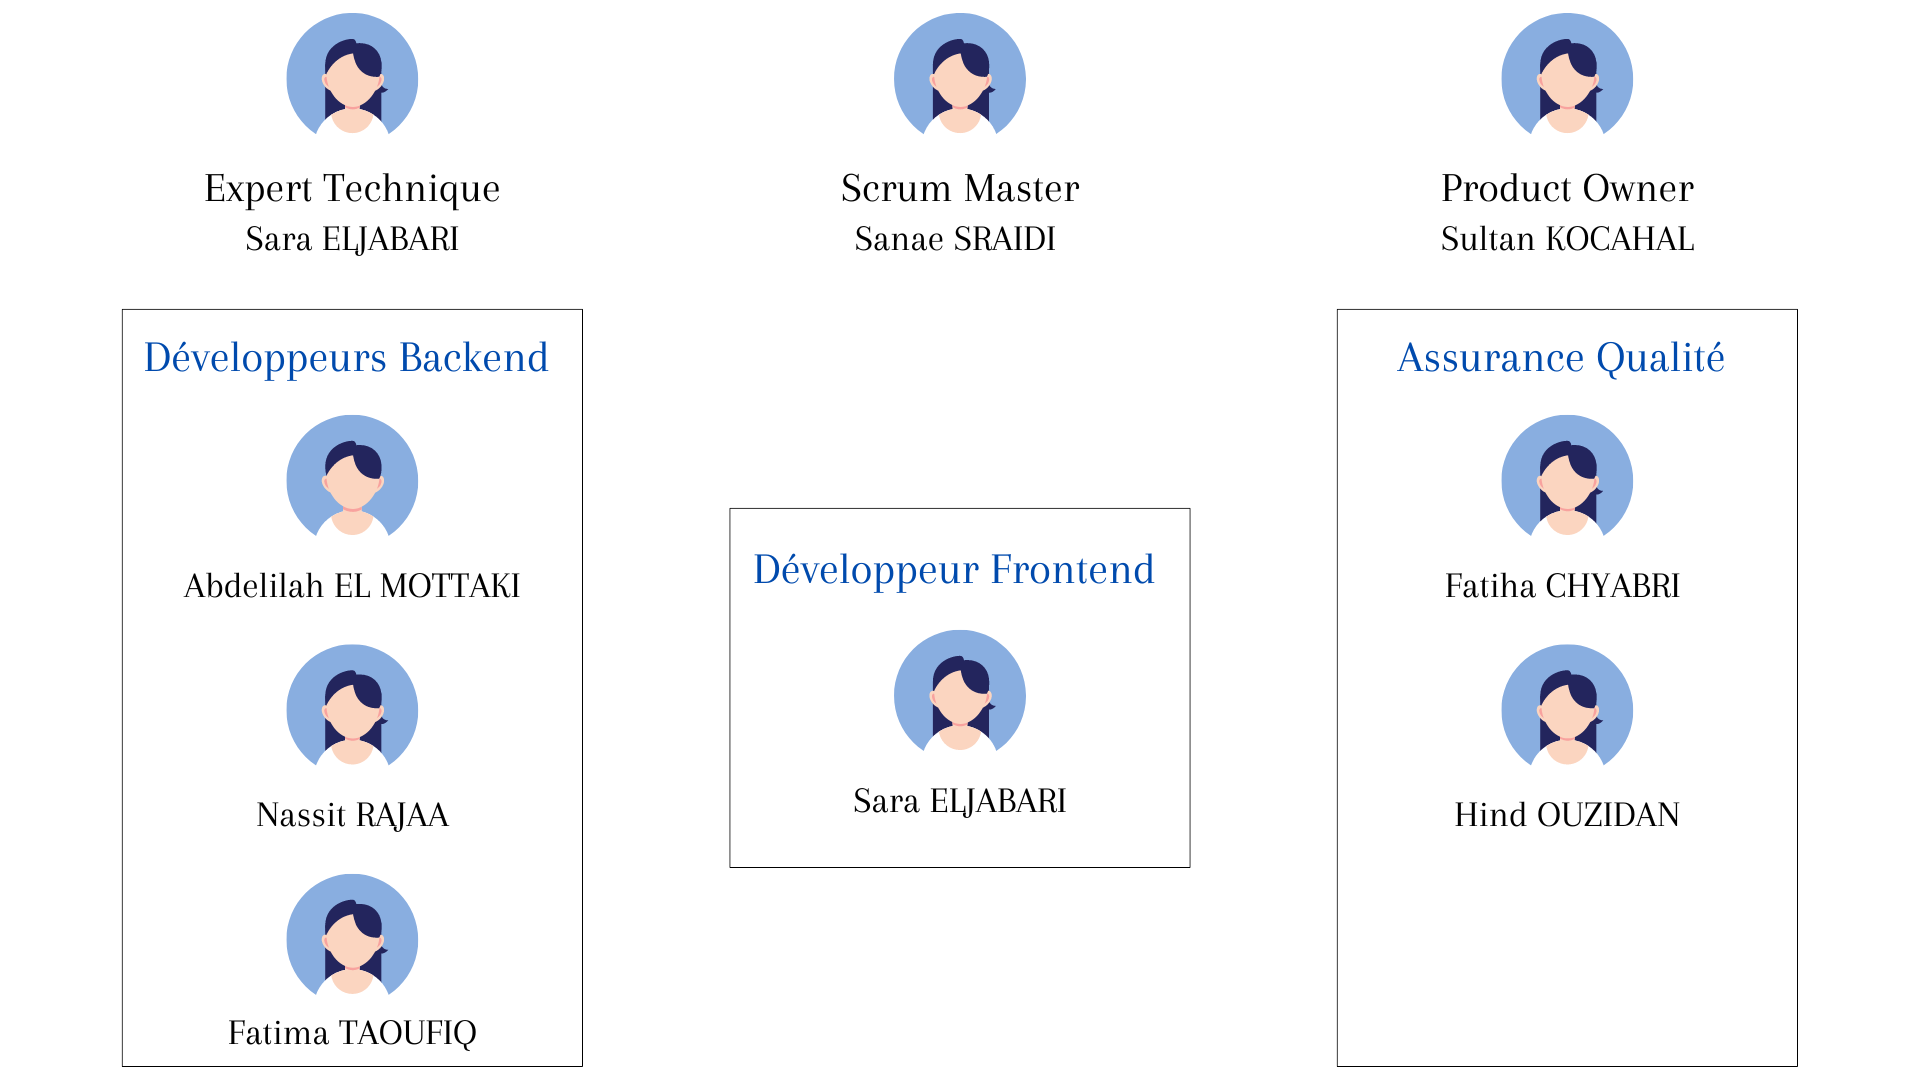
\includegraphics[width=19cm]{Figures/Seasonal Event Team.png}
    \captionof{figure}{Structure de l'équipe Seasonal Event}
    \label{fig:structure_seasonal_event}
\end{center}

\begin{center}
    \centering
    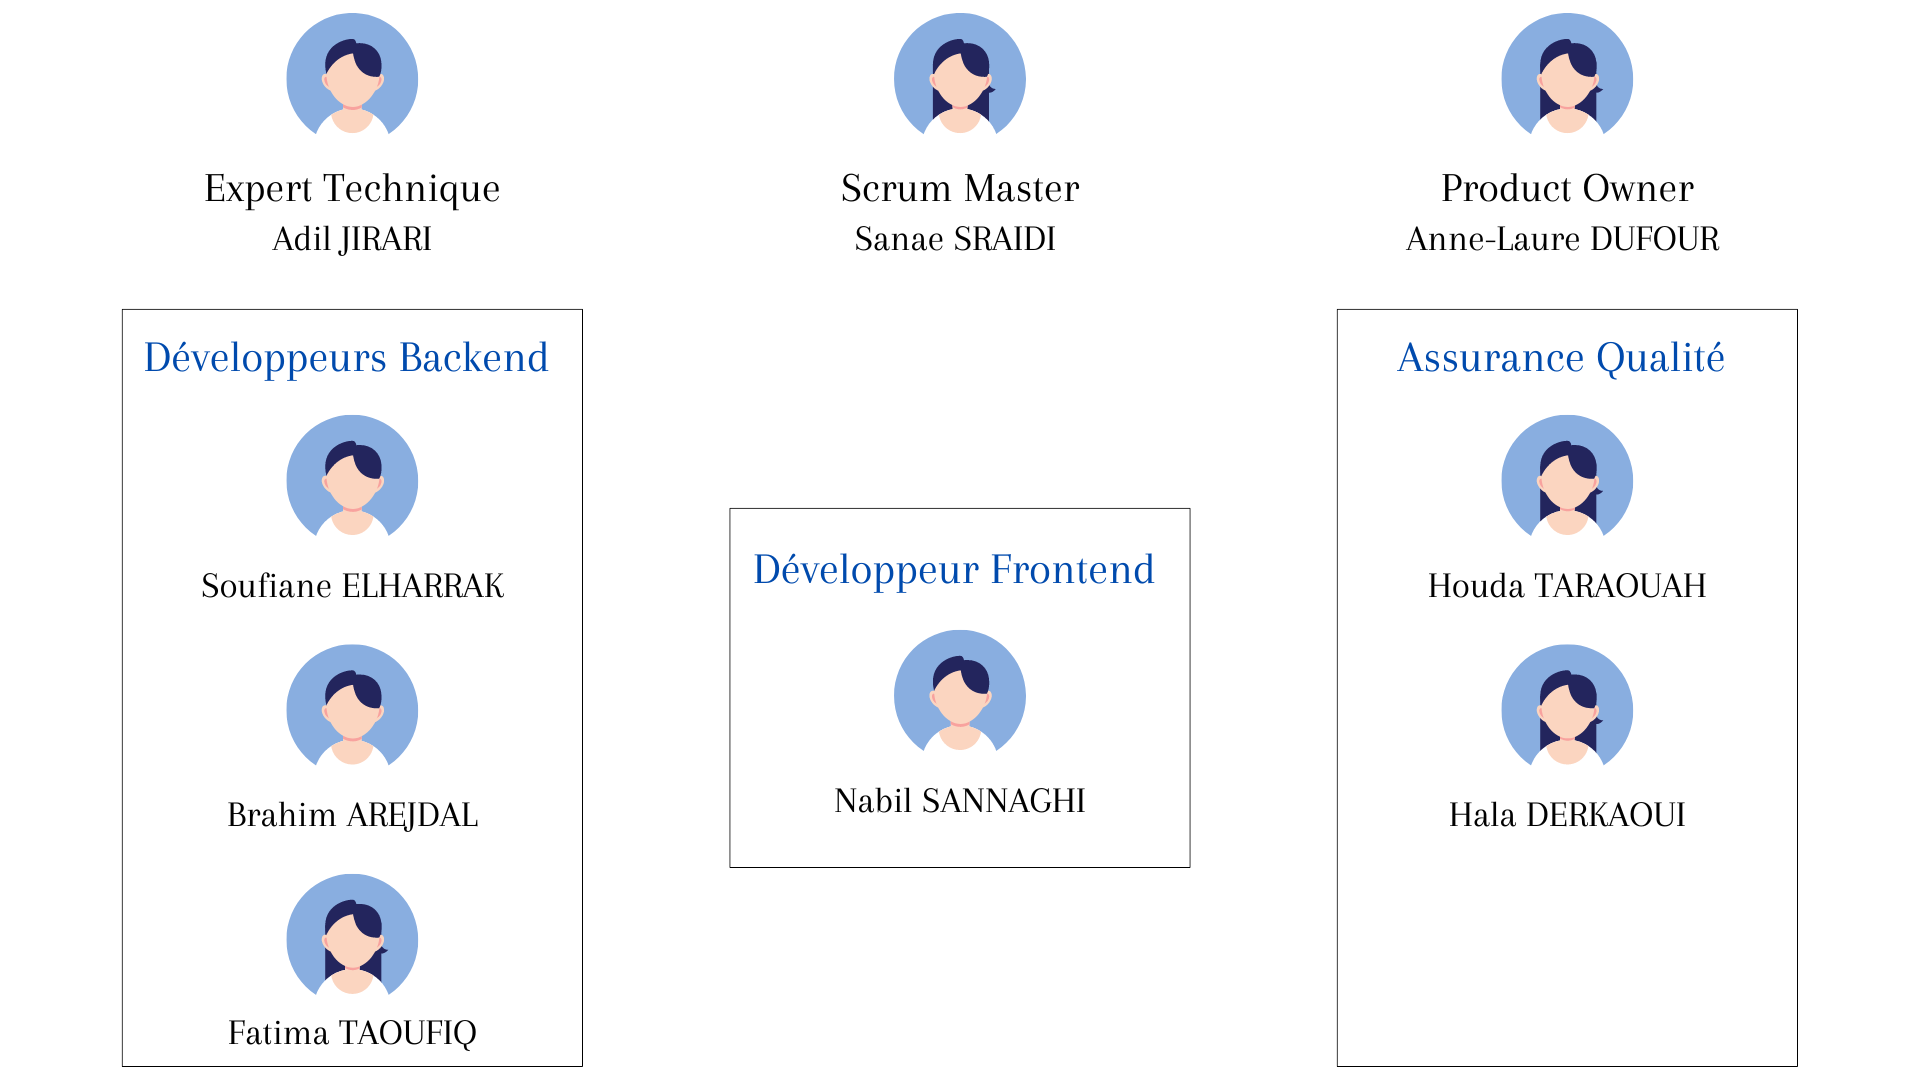
\includegraphics[width=19cm]{Figures/Cart Checkout & Payment.png}
    \captionof{figure}{Structure de l'équipe Cart Checkout \& Payment}
    \label{fig:structure_payment}
\end{center}


\subsection{Méthodologie de travail : Scrum}

Pour assurer une collaboration efficace au sein de l'équipe, nous avons opté pour la méthodologie Scrum, qui se caractérise par une approche itérative et incrémentale. Scrum nous permet de diviser le travail en sprints, des cycles de développement courts et cadencés, généralement de deux à quatre semaines. À la fin de chaque sprint, une version potentiellement livrable du produit est présentée, ce qui favorise la flexibilité et l'adaptation aux changements. Grâce à cette méthode, nous pouvons rester réactifs et ajuster rapidement notre travail en fonction des évolutions des besoins métiers. En intégrant les retours d'expérience du client à chaque itération, nous assurons une satisfaction optimale de ses attentes. Les rôles bien définis, tels que le Scrum Master, le Product Owner, et l'équipe de développement, garantissent une communication claire et une responsabilité partagée. Cette approche nous permet d'être efficaces tout en maintenant un rythme de travail soutenu et structuré.

\subsection{Outils de collaboration}

\subsubsection{Skype}

\begin{figure}[h]
    \centering
    
\includegraphics[scale=0.02]{Logos/Skype-Logo.png} % Replace with the actual filename of the IBM logo image
    \caption{Skype Logo}
\end{figure}

Skype est un outil de communication essentiel qui a facilité le déroulement de mon projet. Il permet d'effectuer des appels téléphoniques et vidéo via Internet, ainsi que le partage d'écran. Pendant toute la durée de mon projet de fin d'études, Skype a joué un rôle crucial en me permettant de maintenir un contact régulier avec mon encadrant, mes collègues et les membres de l'entreprise.

Les appels gratuits entre utilisateurs ont facilité les échanges quotidiens, tandis que la fonction de partage d'écran a été particulièrement bénéfique pour réaliser des présentations et des démonstrations de mon travail en temps réel. Cette fonctionnalité a grandement contribué à la fluidité de nos échanges et à l'efficacité de la communication, éléments essentiels pour la réussite du projet.

En somme, Skype a permis une collaboration efficace et une gestion optimisée des tâches, soutenant ainsi l'avancement et la qualité du projet de fin d’études.

\subsubsection{Git}

\begin{figure}[H]
    \centering
    
\includegraphics[scale=0.5]{Logos/git.png}
    \caption{Logo Git}
\end{figure}

Pour la gestion des versions du code source, nous avons opté pour l'utilisation de Git. Git est un système de contrôle de version décentralisé, largement adopté dans le domaine du développement logiciel.

Ce logiciel libre, sous licence GNU, permet de suivre les modifications apportées au code source tout au long du projet. Grâce à Git, nous avons pu gérer efficacement les différentes versions du code, collaborer en simultané avec plusieurs membres de l'équipe, et assurer une traçabilité précise des changements effectués.

\subsubsection{GitLab}


\begin{figure}[H]
    \centering
    
\includegraphics[scale=0.1]{Logos/gitlab.jpg}
    \caption{Logo GitLab}
\end{figure}

Pour compléter l'utilisation de Git, nous avons également choisi GitLab comme plateforme d'hébergement de code. GitLab offre des outils puissants pour le contrôle de version et la collaboration en équipe. Il permet à tous les membres de l'équipe de travailler ensemble de manière fluide, quel que soit leur emplacement. En centralisant les dépôts de code, GitLab facilite la gestion des contributions, le suivi des problèmes, et les demandes de fusion (merge requests), renforçant ainsi la coordination et l'efficacité du travail collectif.

La figure suivante (\textit{Figure~\ref{fig:client}}) représente une aperçu globale sur l'espace Gitlab 

\section*{Conclusion}
Au cours de ce chapitre, nous avons mis l’accent sur le périmètre de notre projet. Nous avons éclairé
la méthodologie et le planning suivis pour mener ce projet. Nous entamerons dans le chapitre suivant
la phase d’analyse et spécification du système à développer au cours de laquelle nous comprenons en
profondeurs les besoins utilisateurs et construisons ainsi un système qui y répond.

